%\documentclass[handout]{ximera}
\documentclass[nooutcomes]{ximera}

\usepackage{gensymb}
\usepackage{tabularx}
\usepackage{mdframed}
\usepackage{pdfpages}
%\usepackage{chngcntr}

\let\problem\relax
\let\endproblem\relax

\newcommand{\property}[2]{#1#2}




\newtheoremstyle{SlantTheorem}{\topsep}{\fill}%%% space between body and thm
 {\slshape}                      %%% Thm body font
 {}                              %%% Indent amount (empty = no indent)
 {\bfseries\sffamily}            %%% Thm head font
 {}                              %%% Punctuation after thm head
 {3ex}                           %%% Space after thm head
 {\thmname{#1}\thmnumber{ #2}\thmnote{ \bfseries(#3)}} %%% Thm head spec
\theoremstyle{SlantTheorem}
\newtheorem{problem}{Problem}[]

%\counterwithin*{problem}{section}



%%%%%%%%%%%%%%%%%%%%%%%%%%%%Jenny's code%%%%%%%%%%%%%%%%%%%%

%%% Solution environment
%\newenvironment{solution}{
%\ifhandout\setbox0\vbox\bgroup\else
%\begin{trivlist}\item[\hskip \labelsep\small\itshape\bfseries Solution\hspace{2ex}]
%\par\noindent\upshape\small
%\fi}
%{\ifhandout\egroup\else
%\end{trivlist}
%\fi}
%
%
%%% instructorIntro environment
%\ifhandout
%\newenvironment{instructorIntro}[1][false]%
%{%
%\def\givenatend{\boolean{#1}}\ifthenelse{\boolean{#1}}{\begin{trivlist}\item}{\setbox0\vbox\bgroup}{}
%}
%{%
%\ifthenelse{\givenatend}{\end{trivlist}}{\egroup}{}
%}
%\else
%\newenvironment{instructorIntro}[1][false]%
%{%
%  \ifthenelse{\boolean{#1}}{\begin{trivlist}\item[\hskip \labelsep\bfseries Instructor Notes:\hspace{2ex}]}
%{\begin{trivlist}\item[\hskip \labelsep\bfseries Instructor Notes:\hspace{2ex}]}
%{}
%}
%% %% line at the bottom} 
%{\end{trivlist}\par\addvspace{.5ex}\nobreak\noindent\hung} 
%\fi
%
%


\let\instructorNotes\relax
\let\endinstructorNotes\relax
%%% instructorNotes environment
\ifhandout
\newenvironment{instructorNotes}[1][false]%
{%
\def\givenatend{\boolean{#1}}\ifthenelse{\boolean{#1}}{\begin{trivlist}\item}{\setbox0\vbox\bgroup}{}
}
{%
\ifthenelse{\givenatend}{\end{trivlist}}{\egroup}{}
}
\else
\newenvironment{instructorNotes}[1][false]%
{%
  \ifthenelse{\boolean{#1}}{\begin{trivlist}\item[\hskip \labelsep\bfseries {\Large Instructor Notes: \\} \hspace{\textwidth} ]}
{\begin{trivlist}\item[\hskip \labelsep\bfseries {\Large Instructor Notes: \\} \hspace{\textwidth} ]}
{}
}
{\end{trivlist}}
\fi


%% Suggested Timing
\newcommand{\timing}[1]{{\bf Suggested Timing: \hspace{2ex}} #1}




\hypersetup{
    colorlinks=true,       % false: boxed links; true: colored links
    linkcolor=blue,          % color of internal links (change box color with linkbordercolor)
    citecolor=green,        % color of links to bibliography
    filecolor=magenta,      % color of file links
    urlcolor=cyan           % color of external links
}

\title{Lines in Triangles}
\author{Bart Snapp and Brad Findell}

\outcome{Learning outcome goes here.}

\begin{document}
\begin{abstract}
  We think about some special lines in triangles. 
\end{abstract}
\maketitle

\begin{teachingnote}
This preactivity for Isosceles Bisectors is about (1) the meanings of median, altitude, angle bisector, and perpendicular bisector; (2) drawing them carefully with protractor and ruler; and (3) noticing that they are four different lines in a general triangle. 
\end{teachingnote}

Two copies of a triangle are shown below.   In each triangle, \textbf{draw carefully} the designated lines.  \emph{Construction is not necessary:  Careful measurements are allowed.}

\begin{problem}
In the triangle below, draw the median from $B$ to $\overline{AC}$, the altitude from $B$ to $\overline{AC}$, the angle bisector of $\angle B$, and the perpendicular bisector 
of $\overline{AC}$.  

%\begin{enumerate}
%\item Median from $B$ to $\overline{AC}$
%\item Altitude from $B$ to $\overline{AC}$
%\item Angle bisector of $\angle B$
%\item Perpendicular bisector of $\overline{AC}$
%\end{enumerate}
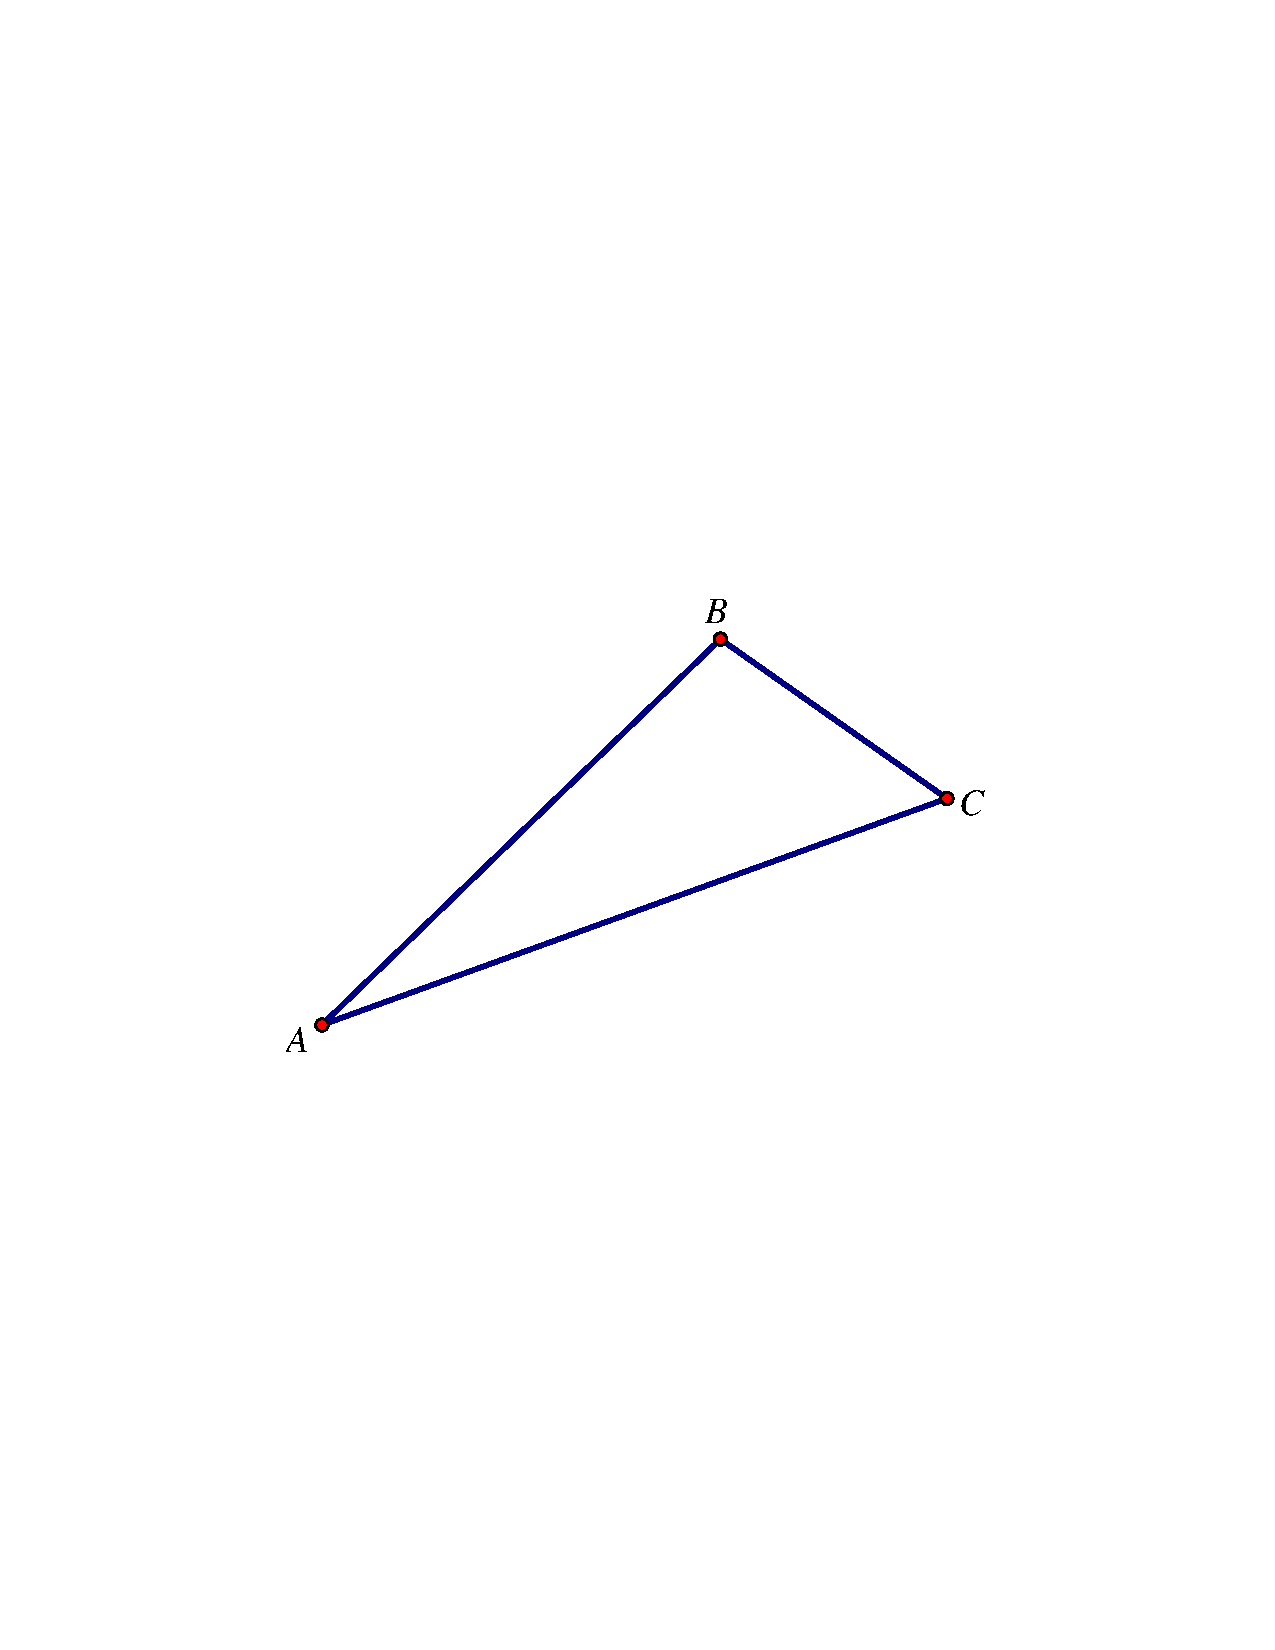
\includegraphics[scale=0.9]{obtuseTriangle.pdf}
\vfill
\end{problem}

\newpage
\begin{problem}
In the triangle below, draw the median from $C$ to $\overline{AB}$, the altitude from $C$ to $\overline{AB}$, the angle bisector of $\angle C$, and the perpendicular bisector of $\overline{AB}$. 

%\begin{enumerate}
%\item Median from $C$ to $\overline{AB}$
%\item Altitude from $C$ to $\overline{AB}$
%\item Angle bisector of $\angle C$
%\item Perpendicular bisector of $\overline{AB}$
%\end{enumerate}
%
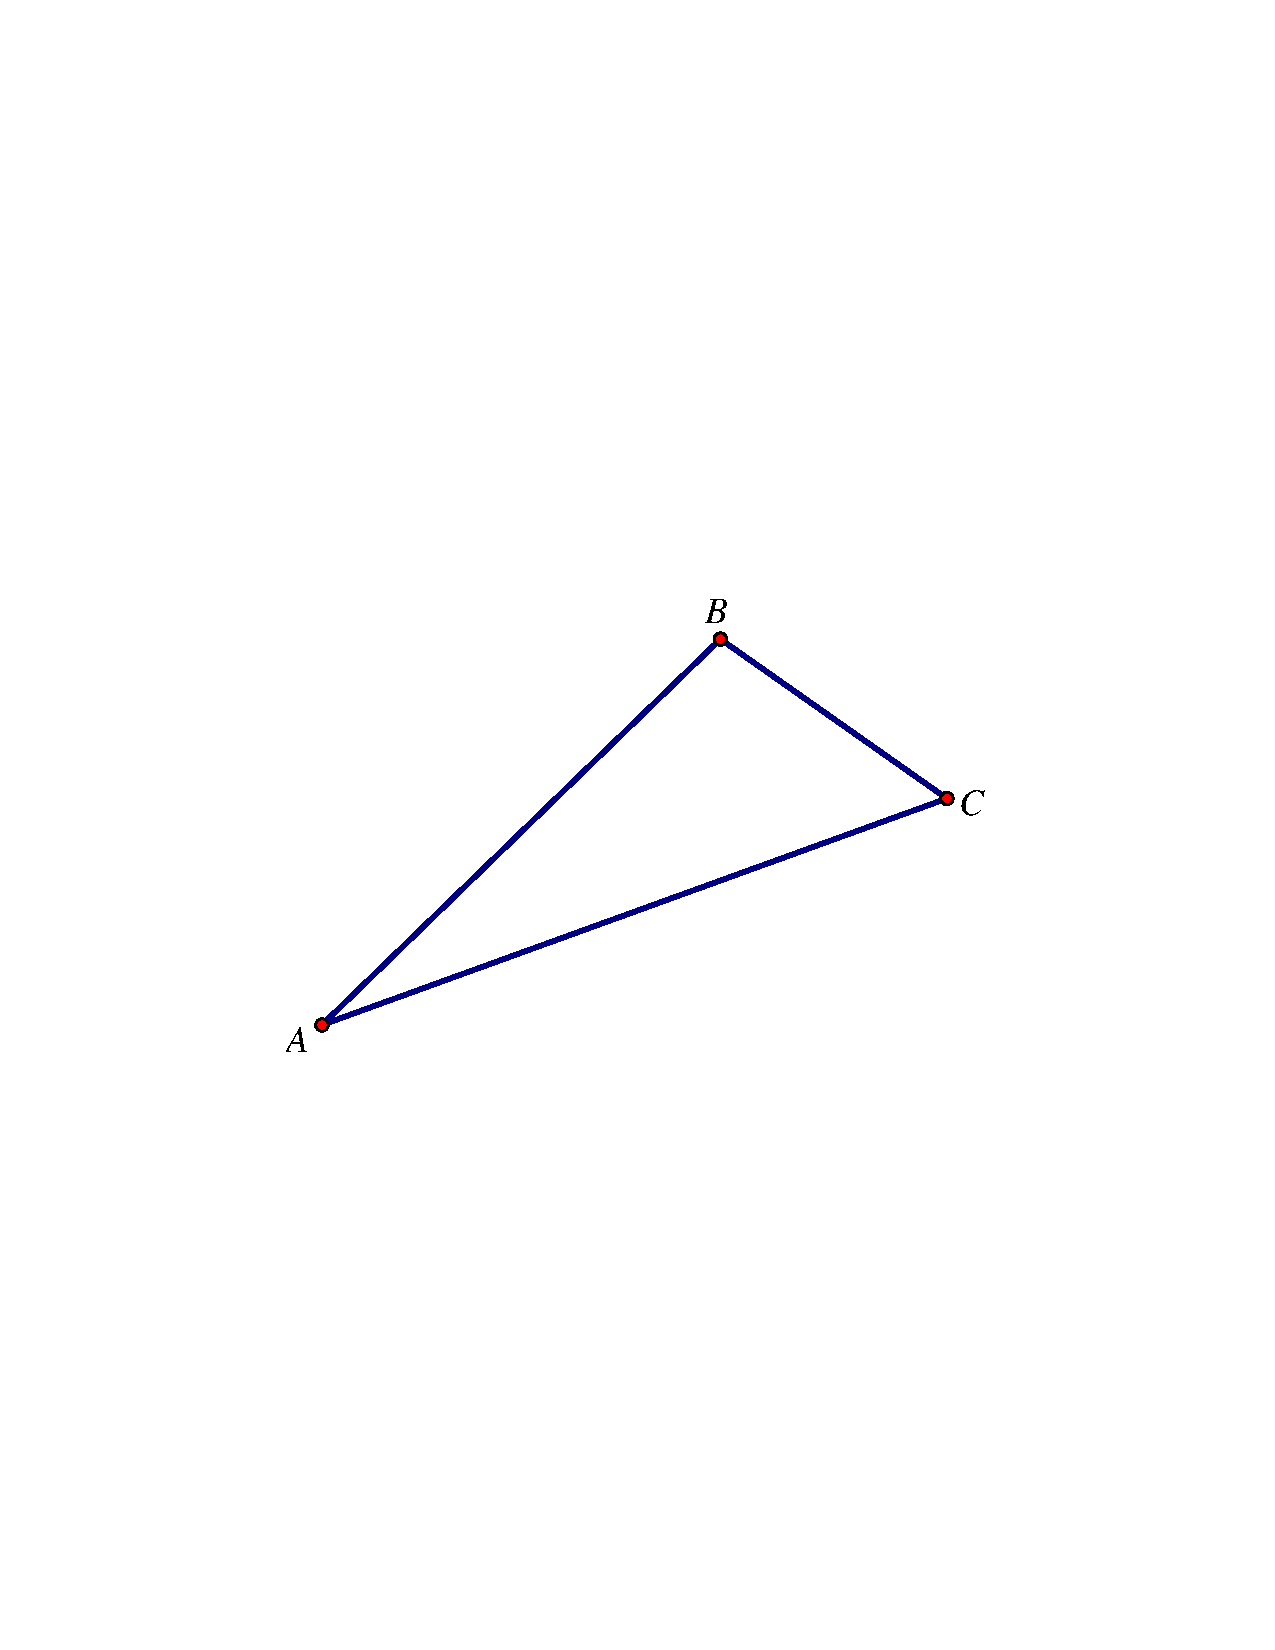
\includegraphics[scale=0.9]{obtuseTriangle.pdf}
\end{problem}


\begin{problem}
In each triangle, you should have drawn four different lines.  What might you say about a triangle for which two or more of these lines turn out to be the same?  
\vfill
\end{problem}

\end{document}
